\chapter{Equilibre Statique Du Kite}
\label{ch:Ch1}

%%%%%%%%%%%%%%%%%%%%%%%%%%%%%%%%%%%% SECTION 1
\section{\textbf{$X_{T}$}} 
\label{sec:Ch1.1}

le point d'application d'un effort est une notion importante. Si celui de l'effort aérodynamique et du poids sont couramment utilisés, le point d'application de la tension des lignes influence beaucoup les performances d'un kite. De plus, le bridage d'un kite change considérablement la façon dont se répartie la tension dans les lignes et l'angle d'équilibre au zénith d'un kite. Ainsi, afin de capturer l'influence du bridage sur les performances d'un kite, on définit $X_T$ comme étant \textbf{le point d'intersection entre la corde moyenne d'un kite et l'axe de la tension des lignes}. Ainsi, $X_T$ permet de lié la géométrie du bridage et son influence sur la dynamique du kite.  \\

\begin{figure}[H]
    \centering
    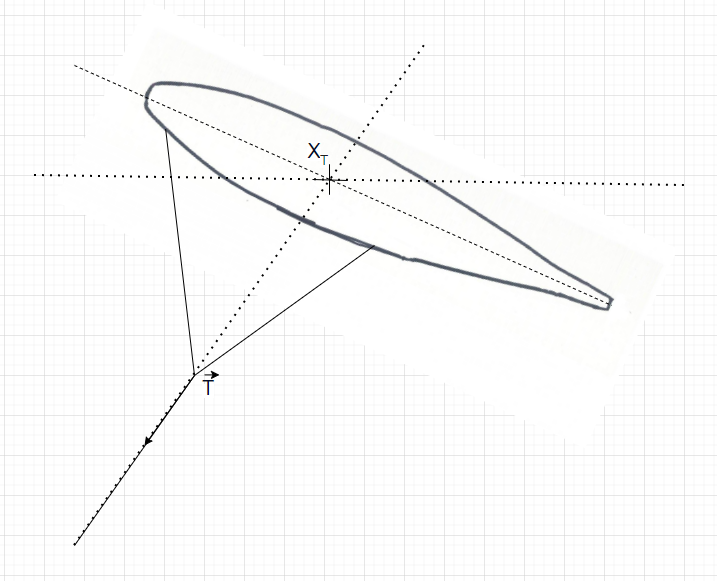
\includegraphics[width=0.5\textwidth]{Pics/01 - xt et towpoint/Xt.png}  
    \caption{Xt}
    \label{fig:Xt}
\end{figure}

Isoler les ensembles \{kite\} et \{kite+bridage\} permet de montrer $X_T$ est le point d'application de l'ensemble du bridage, le long de la corde. En effet :

Pour l'équilibre des moments appliqué à l'ensemble \{kite\}, en le $X_T$ :
\begin{equation}
    F_{Poid}(x_G-x_T)+F{aero}(x_{aero}-x_T) = 0
\end{equation}

Pour l'équilibre des moments appliqué à l'ensemble \{kite+bridage\}, $X_T$:
\begin{equation}
    F_{Poid}(x_G-x_T) + F{aero}(x_{aero}-x_T) + \sum_{i=A}^{D} F_{ligne i}(x_{ligne i}-x_T)= 0
\end{equation}

D'où : 
\begin{equation}
    \sum_{i=A}^{D} F_{ligne i}(x_{ligne i}-x_T)= 0
\end{equation}

Ce qui, par définition, montre que \textbf{$X_T$ est le point d'application de la résultante de tension de l'ensemble du bridage projeté sur la corde.}




%%%%%%%%%%%%%%%%%%%%%%%%%%%%%%%%%%%% SECTION 2
\section{\textbf{Tow Point}} 
\label{sec:Ch1.2}

On définit le Tow Point par \textbf{le projeté orthogonal du point d'attache entre les lignes et le bridage sur la corde moyenne du kite}. 

\begin{figure}[H]
    \centering
    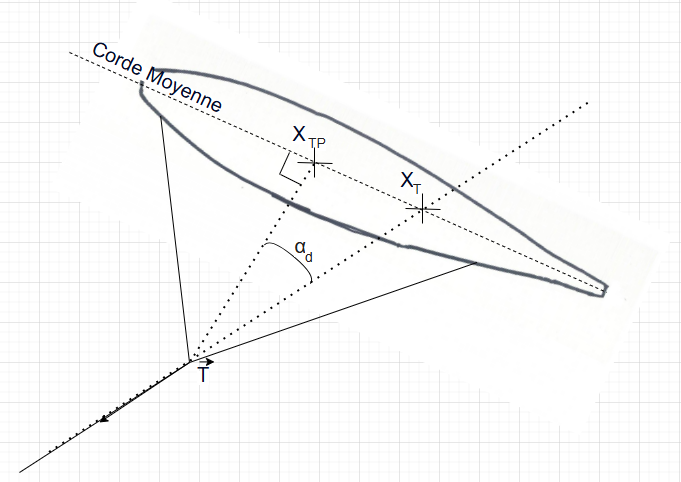
\includegraphics[width=0.5\textwidth]{Pics/01 - xt et towpoint/xtp.png}  
    \caption{Différence entre $x_{TP}$ et $x_T$}
    \label{fig:Xtp}
\end{figure}

Le schéma \ref{fig:Xtp} montre que le towpoint ($x_{TP}$) et $x_T$ forment un angle $\alpha_0$ avec le point d'attache entre les lignes et le bridage. Ainsi, dans le cas où les lignes forment un angle de $\frac{\pi}{2}$ avec la corde moyenne du kite, Tow Point et $x_T$ sont confondus. 

De plus, $x_{TP}$ est purement géométrique là où $x_T$ lie géométrie et aérodynamique.

On peut lier ces deux positions par la relation suivante : 

\begin{equation}
    x_{TP} = x_T + d * tan(\alpha_0)
    \label{eq:Xtp}
\end{equation}

où d est la distance du point d’attache entre les lignes et le bridage à la corde moyenne, divisé par la corde profil.

%%%%%%%%%%%%%%%%%%%%%%%%%%%%%%%%%%%% SECTION 3
\section{\textbf{Equilibre Statique Du Kite}} 
\label{sec:Ch1.3}

\begin{figure}[H]
    \centering
    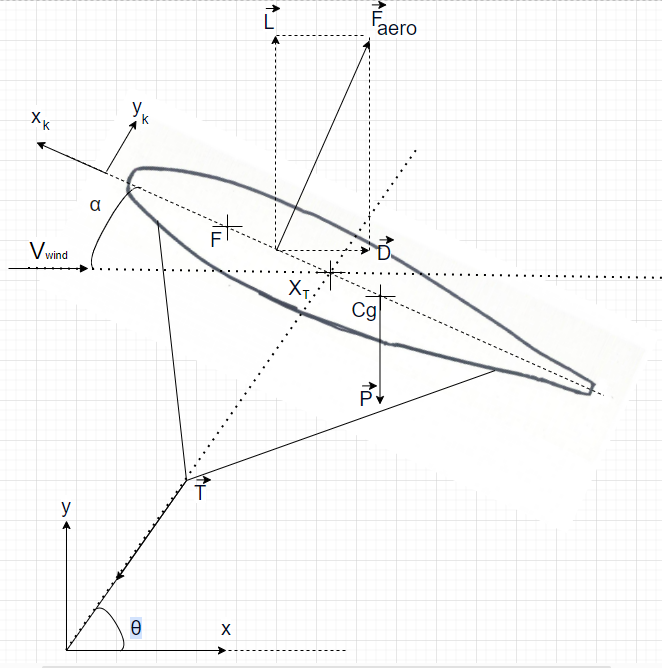
\includegraphics[width=0.5\textwidth]{Pics/01 - xt et towpoint/Equilibre Kite.png}  
    \caption{Equilibre du kite}
    \label{fig:Equilibre du kite}
\end{figure}

On écrit l'équilibre statique de \{kite+bridage\}, en $X_T$ du kite : 

\begin{equation}
    \begin{cases}
        L = P + T sin(\theta) \\
        D = T cos(\theta) \\
        0 = C_{M_0} + (x_T - x_F) (L cos(\alpha) + D sin(\alpha)) - P cos(\alpha) (x_T - x_G)
    \end{cases}
\end{equation}

Ainsi, en considérant $\alpha << 1$, on a :

\begin{equation}
    \begin{cases}
    \frac{L-P}{D} = tan(\theta) \\
    \theta = \frac{\pi}{2} - \alpha + \alpha_0 \\
    x_T = \frac{L x_F - P x_G -C_{M_0}}{L - P}
    \end{cases}
    \label{eq:Xt}
\end{equation}
    
Il semblerait donc que le calcul (CFD, VSM, ...) des polaires aérodynamiques ($L(\alpha)$ et $D(\alpha)$) permettent de trouver le $X_T$ optimal afin d'optimiser la finesse au zénith. 

\textit{Exemple : }
Pour $\alpha_{optimal} = 21^\circ$, $C_D = 0.19$ et $C_L = 1.35$, on trouve en appliquant l'équation \ref{eq:Xt} : \\

\begin{equation}
    \begin{cases}
    \alpha_0 =  -12^\circ\\
    \theta = 81^\circ\\
    x_T = 0.22
    \end{cases}
    \label{eq:Xt results}
\end{equation}

avec $P = 21 kg$, $x_F = 0.25$, $x_G = 0.5$,$\frac{1}{2} \rho S v^2 = \frac{1}{2} 1.225 * (50m^2) * (14 * 0.514 m/s)^2$  et $C_{M_0} = 0$ \\

De plus, avec  $d = \frac{6.9 m}{4.56 m} = 1.51 m$ pour une $50m^2$ (d'après SurfPlan). On a finalement :\\
$x_{TP} = -0.10 $

Ce resultat semble correct en ordre de grandeur (comme celui de $x_{TP}$) mais pas "exacte"; comparé aux observations expérimentales. On comprend donc l'importance de déterminer chaque grandeur, notamment les coefficients aérodynamiques, avec davantage de précision !

%%%%%%%%%%%%%%%%%%%%%%%%%%%%%%%%%%%% SECTION 4
\section{\textbf{Condition d'existence de l'équilibre du kite}} 
\label{sec:Ch1.4}

\subsection{Angle d'élévation minimal} 
\label{sec:Ch1.4.1}

\subsection{Angle d'élévation maximal}
\label{sec:Ch1.4.2}


%%%%%%%%%%%%%%%%%%%%%%%%%%%%%%%%%%%% SECTION 5
\section{\textbf{Stabilité du kite}} 
\label{sec:Ch1.5}